\documentclass[10pt]{article}
\usepackage{tmlr}
\usepackage{hyperref}
\usepackage{url}
\usepackage{booktabs}
\usepackage{graphicx}

\title{The Benchmark Cannot Tell You Which Probes Work}

\author{\name Anonymous \email anonymous@example.com \\
      \addr Withheld for review}

\newcommand{\fix}{\marginpar{FIX}}
\newcommand{\new}{\marginpar{NEW}}

\def\month{08}
\def\year{2026}
\def\openreview{\url{https://openreview.net/forum?id=XXXXXXXXXX}}

\begin{document}
\maketitle

\begin{abstract}

A linear probe trained on a language model's hidden states separates true statements from false ones and reports a high AUROC, which is read as evidence that the model represents truth internally. In the datasets these probes are trained on, true statements are also the ordinary ones, so a probe that learned only ``familiar means true'' would report the same number. We built a corpus of 608 statements that crosses truth against entity frequency and evaluated 18 models from 70M to 12B parameters. Trained the standard way and then stripped of every false statement, our probes separate common entities from rare ones among statements that are all true at AUROC 0.766 to 0.961. Truth is constant throughout, so that signal is not truth. Trained on the diagonal where the two agree and tested where they disagree, the same probes range from 0.08 to 0.89 while reporting 0.76 to 1.00 on the split the field publishes. Across 98 probe-model pairs spanning six architectures from four groups, the published score predicts the off-diagonal AUROC at Spearman 0.198 [-0.005, 0.366], and 48 of the 98 fall below chance. On a second corpus whose falsehoods are a model's own errors rather than ours, no model of the 18 exceeds chance, the best reaching 0.447. A sampling-based detector on the same models detects their errors at 0.758 to 0.822 and shows nothing on the frequency contrast, 0.500 to 0.514, so this is a property of reading hidden states rather than of model uncertainty. The alignment between truth and familiarity is not all-or-nothing: it is partial in a published dataset and total in corpora built without a check for it, and the standard protocol reports the same high number across that whole range. We release the gates, which flag four of our own five corpora.

\emph{Draft for TMLR. Every number traces to a committed artifact in \texttt{results/}. Nothing below was typed from memory. Unless stated otherwise, results are on corpus \texttt{v44b4126cba1c} (n = 608).}

\end{abstract}
\section{Introduction}

The claim under audit is that a language model's hidden states encode whether a statement is true, and that a small classifier reading those states detects falsehood. Azaria and Mitchell report 71-83\% accuracy across base models with this method \citep{azaria2023internal}, and the approach has been extended in several directions since \citep{marks2023geometry,burns2023discovering,burger2024truth}. There is a second reading of the same evidence. In the datasets these classifiers are trained and tested on, true statements are also the ordinary ones and false statements are also the odd ones, so a classifier that learned only ``familiar means true'' would produce the same numbers. We can now put a figure on how far that alternative goes. Take our classifiers trained the standard way, discard every false statement, and ask them to separate common entities from rare ones among statements that are all true: AUROC \textbf{0.766 to 0.961} across 18 models, mean 0.909. Truth is held constant throughout. Whatever produces those scores is not truth.

To separate the two, we crossed them. Each statement is true or false and is about a common or a rare entity, giving four cells: true-common, true-rare, false-common, false-rare. Standard datasets sit almost entirely on the true-common and false-rare diagonal. We train there, exactly as the field does, and test on the other two cells, where familiarity and truth point in opposite directions. On the diagonal our classifiers score 0.76 to 1.00 across 18 models from 70M to 12B parameters. On the off-diagonal the same classifiers, at the same layers, range from \textbf{0.08 to 0.89}. A classifier that is useless on the off-diagonal test and one that works are separated by little on the number that gets published.

That result is about our training distribution, and we ran the experiment that says so. Training instead on 9,270 statements from Azaria and Mitchell's released files, decontaminated against our corpora because 75.3\% of our authored items appear verbatim in them, the off-diagonal AUROC is \textbf{0.882 to 0.997} across four models, so there is no collapse. Their row-swap construction roughly preserves entity frequency across truth, and three of the four models trained on it read frequency far more weakly than ours do, though pythia-6.9b reads it at 0.891 and is the exception. What those probes learn is clearest when the falsehoods change shape. Mean probe scores, not AUROC: on our authored false-common cell, built by swapping the country in a true statement, they place the items at 0.014 to 0.126. On a false-common cell whose items are errors a model actually produced, the same weights place them at \textbf{0.287 to 0.556}. They reject the falsehoods whose construction they were trained on and have close to no opinion about the ones they were not.

The second corpus is worth stating carefully because it is the one most likely to be misread. Its falsehoods are greedy-decoded answers from Qwen2.5-1.5B-Instruct, checked against a multi-valued Wikidata gazetteer and kept only where the model's answer is wrong. That model is not among the 18 we evaluate, though its base model is, and we do not claim these are self-beliefs: a probe reads the hidden states of a different model from the one that erred. The claim is narrower and does not need self-belief. A classifier reading hidden states cannot mark false the statements models find plausible, and a model's greedy errors are drawn from exactly that set. Across 18 models the per-cell means are 0.904 true-common, 0.254 true-rare, \textbf{0.661 false-common}, 0.087 false-rare. Probes rate a model's errors above true statements about rare entities. Not one of the 18 exceeds chance on the off-diagonal split; the best is 0.447, while the same probes score 0.88 to 1.00 on the diagonal. A frequency control rules out gross composition confounding: false items are slightly rarer than true ones overall (-0.122 log10 typicality), so the corpus is not stacked toward the effect in aggregate.

We had an account of why the collapse is as large as it is, and it survives on one corpus only. Recoverability, meaning how much truth signal a classifier trained on all four cells can extract at a given layer, measured as a partial regression coefficient with typicality and fragmentation held out, predicts the off-diagonal score at r = 0.82 on the authored corpus, with a hinge shape preferred over linear and step fits by AIC. On the harvested corpus it does not replicate: r = 0.49, with a confidence interval crossing zero. The mechanism is a claim about falsehoods we wrote.

Two boundaries. A sampling-based detector on the same models detects their errors at 0.758 to 0.822 and shows nothing on the frequency contrast, 0.500 to 0.514, so the problem belongs to reading hidden states rather than to models being uncertain about rare things. And we are not exempt. Five of our own corpus versions were built and four had defects we found ourselves: a topic that predicted truth, a frequency axis that was 91\% failed network calls, duplicate sentences, and an edit imbalance worth 0.075 AUROC on its own. All four are now build-time gates, along with a fifth that checks the crossing itself, which nothing has yet tripped. The released checker flags our own withdrawn corpora. Everything here rests on 608 authored and 140 harvested items, English, one sentence pattern per topic.

\section{What we built}

A corpus of 608 statements crossing truth against entity frequency: 152 in each of four cells, drawn from three domains (cities, companies, inventions).

\begin{figure}[t]
\centering
\small
\begin{tabular}{@{}l|p{0.36\linewidth}|p{0.36\linewidth}@{}}
& \textbf{Common} & \textbf{Rare} \\
& \footnotesize high pretraining frequency & \footnotesize low pretraining frequency \\
\hline
\rule{0pt}{3.0ex}\textbf{True} & \textbf{TT} \emph{(diagonal, trained)} & \textbf{TA} \emph{(off-diagonal, tested)} \\
& \footnotesize ``Paris is a city in France.'' & \footnotesize ``Catape is a city in Angola.'' \\[1.0ex]
\hline
\rule{0pt}{3.0ex}\textbf{False} & \textbf{FT} \emph{(off-diagonal, tested)} & \textbf{FA} \emph{(diagonal, trained)} \\
& \footnotesize ``Monywa is a city in Brazil.'' & \footnotesize ``Biba is a city in Tuvalu.'' \\[0.6ex]
\end{tabular}
\caption{The 2x2 design. Standard datasets occupy the TT/FA diagonal, where truth and entity frequency agree; the TA/FT off-diagonal is where they disagree and is the only place the question can be asked.}
\label{fig:design}
\end{figure}

The four cells are the design. \textbf{TT} is true and common. \textbf{TA} is true but rare, the Guyana case. \textbf{FT} is false but fluent and ordinary sounding, the confident lie. \textbf{FA} is false and odd. Standard benchmarks live almost entirely on the TT/FA diagonal, where truth and typicality agree. The off diagonal is where they disagree, and it is the only place the question can be asked.

Typicality is entity frequency from pretraining corpus counts, not perplexity. We preregistered a plan to measure typicality three ways and check that they agree. Two of the three are measurable without circularity, and they do not agree, which settled the choice for us.

Frequency and reference perplexity are close to unrelated on this corpus: Spearman 0.058, p = 0.16. They also load on different things. Frequency separates typical from atypical items by 1.083 standard deviations and separates true from false by 0.032, so it tracks familiarity and carries almost no truth signal. Perplexity does the reverse, separating true from false by 1.172 standard deviations and typical from atypical by 0.036. Median reference perplexity is 17.2 for common true statements and 85.0 for odd false ones, while within a truth class it barely moves, 17.2 against 21.8 for true items and 69.0 against 85.0 for false ones. A corpus built on the perplexity axis would have sorted mostly by truth and left the cell this study depends on empty. The third measure we planned, the model's own probability for the claim, is excluded as circular: it is read from the same network the probe reads.

The axes are crossed within each domain, which matters more than it sounds. Median log frequency by cell: cities 6.65 / 5.40 / 6.71 / 5.33 for TT / TA / FT / FA; companies 7.18 / 6.03 / 7.15 / 6.04; inventions 4.34 / 2.38 / 4.37 / 2.15. Truth does not move with frequency inside a domain. Only the cell label does. Pooled across the corpus, Cliff's delta between typical and atypical is 0.683 on true items and 0.697 on false items, both with p below 1e-24.

Five properties are enforced at build time rather than checked afterwards, and \texttt{finalize()} refuses to write a corpus that violates any of them.

\begin{itemize}
\item No statement appears twice.
\item No domain exceeds half the corpus. Cities is exactly 50.0\%, companies 26.3\%, inventions 23.7\%.
\item \texttt{edited} is drawn 50/50 inside every cell, so P(edited) is 0.500 in TT, TA, FT and FA alike.
\item No metadata field recoverable from the statement text predicts truth off diagonal after learning the association on the diagonal.
\item A domain that cannot fill all four cells is dropped whole rather than contributing to some.
\end{itemize}

The hidden state canaries pass: a probe predicting ``was this edited'' from activations reaches 0.481 with a confidence interval of [0.373, 0.580], and a probe predicting truth from tokenization features alone reaches 0.417 [0.318, 0.506]. Both intervals contain chance.

\subsection{What we got wrong first, and why the corpus looks like this}

Four earlier corpora produced clean, large, cross model effects that we believed at the time. Each was an artifact of our own construction, and each is worth stating because the checks that catch them are cheap and are now released.

The first ranked frequency terciles across pooled domains. Because domains had different frequency profiles, the diagonal ended up 32\% non cities among true items and 0\% among false ones, while the off diagonal reversed that exactly. ``Non city implies true'' was a perfect shortcut in training that inverted at test, so a probe reading nothing but topic scored below chance off diagonal. We reported that as a typicality confound for three weeks. Holding domain fixed removed the whole effect.

The second was worse and simpler. The frequency cache recorded failed API calls as \texttt{count = 0}. Because the endpoint rate limits, 2627 of 2884 entities, or 91\%, were stored as having zero occurrences. Amman's real count is 1,183,125. Paris is 58,070,155. Both were zero. The typicality axis was not entity frequency at all. It was whether the network call happened to succeed, which correlated with domain, which produced the first artifact. One bug, both failures.

The third passed both of those gates and still carried a defect. Seventy of its 696 rows were exact duplicate statements, concentrated almost entirely in the two true cells, because a truth preserving swap could land on a string already present as an original. Per cell counts were equal in rows and unequal in distinct statements, 141 / 139 / 174 / 172. Forty four of the duplicated statements carried contradictory \texttt{edited} flags, so about one in seven of the edit canary's rows was unlearnable by construction, which biases that canary toward passing.

The fourth is the subtlest and we only found it by running an invariant test that had been in the repository since July. The generator left the FA cell edit heavy, 0.578 against roughly 0.42 elsewhere. Since the training diagonal is TT plus FA, ``edited'' predicted false in training and predicted nothing off diagonal. That is the same signature as the confound under study: a shortcut that works in distribution and disappears off it. Using the \texttt{edited} flag itself as the predictor, which bounds what any probe reading provenance perfectly could extract, it was worth a gap of +0.075 before a probe read a single hidden state. Small next to the large gaps, but larger than the small ones, which is exactly where it mattered.

The corpus described above is the fifth attempt. On it, that same bound is \textbf{+0.0000}: a perfect edit shortcut scores 0.500 on the diagonal and 0.500 off it.

\section{The result}

We train each probe the way the field does, on the diagonal where truth and typicality agree, and then evaluate it two ways. On a held out diagonal split, which is what gets reported. And on the off diagonal only, which is what the probe is worth when it can no longer lean on the correlation.

\begin{table}[t]
\centering
\small
\resizebox{\linewidth}{!}{%
\begin{tabular}{lrrrr}
\toprule
\textbf{Model} & \textbf{In-distribution} & \textbf{Off-diagonal AUROC} & \textbf{Gap [95\% CI]} & \textbf{Recoverability} \\
\midrule
Pythia-160m & 0.761 & 0.213 [0.16, 0.27] & +0.548 [0.412, 0.666] & $-$0.072 \\
Pythia-70m & 0.802 & 0.253 [0.20, 0.31] & +0.549 [0.407, 0.667] & $-$0.026 \\
Pythia-2.8b & 0.894 & 0.120 [0.08, 0.16] & +0.773 [0.678, 0.851] & 0.053 \\
Pythia-410m & 0.912 & 0.127 [0.09, 0.17] & +0.786 [0.699, 0.857] & 0.122 \\
Pythia-1b & 0.908 & 0.079 [0.05, 0.11] & +0.829 [0.740, 0.899] & 0.166 \\
Pythia-1.4b & 0.908 & 0.236 [0.19, 0.29] & +0.672 [0.580, 0.754] & 0.373 \\
Pythia-6.9b & 0.967 & 0.122 [0.09, 0.16] & +0.845 [0.784, 0.896] & 0.487 \\
Qwen2.5-0.5B & 0.952 & 0.151 [0.11, 0.19] & +0.802 [0.731, 0.860] & 0.543 \\
Pythia-12b & 0.960 & 0.171 [0.13, 0.22] & +0.789 [0.716, 0.848] & 0.585 \\
Qwen2.5-1.5B & 0.991 & 0.449 [0.39, 0.51] & +0.542 [0.474, 0.608] & 0.836 \\
Qwen2.5-3B & 0.989 & 0.536 [0.47, 0.60] & +0.454 [0.383, 0.516] & 0.854 \\
Qwen2.5-7B & 0.998 & 0.682 [0.62, 0.74] & +0.316 [0.254, 0.378] & 0.865 \\
Gemma-2-2b & 0.996 & 0.761 [0.71, 0.81] & +0.235 [0.179, 0.289] & 0.868 \\
Qwen2.5-7B-Instruct & 0.994 & 0.708 [0.65, 0.76] & +0.286 [0.229, 0.344] & 0.871 \\
Llama-3.1-8B & 0.990 & 0.641 [0.58, 0.71] & +0.349 [0.284, 0.416] & 0.894 \\
Gemma-2-9b-it & 0.971 & 0.888 [0.85, 0.92] & +0.083 [0.015, 0.131] & 0.894 \\
Llama-3.1-8B-Instruct & 0.995 & 0.862 [0.82, 0.90] & +0.133 [0.088, 0.175] & 0.899 \\
Gemma-2-9b & 0.990 & 0.823 [0.77, 0.87] & +0.167 [0.115, 0.216] & 0.917 \\
\bottomrule
\end{tabular}}
\end{table}

\begin{figure}[t]
\centering
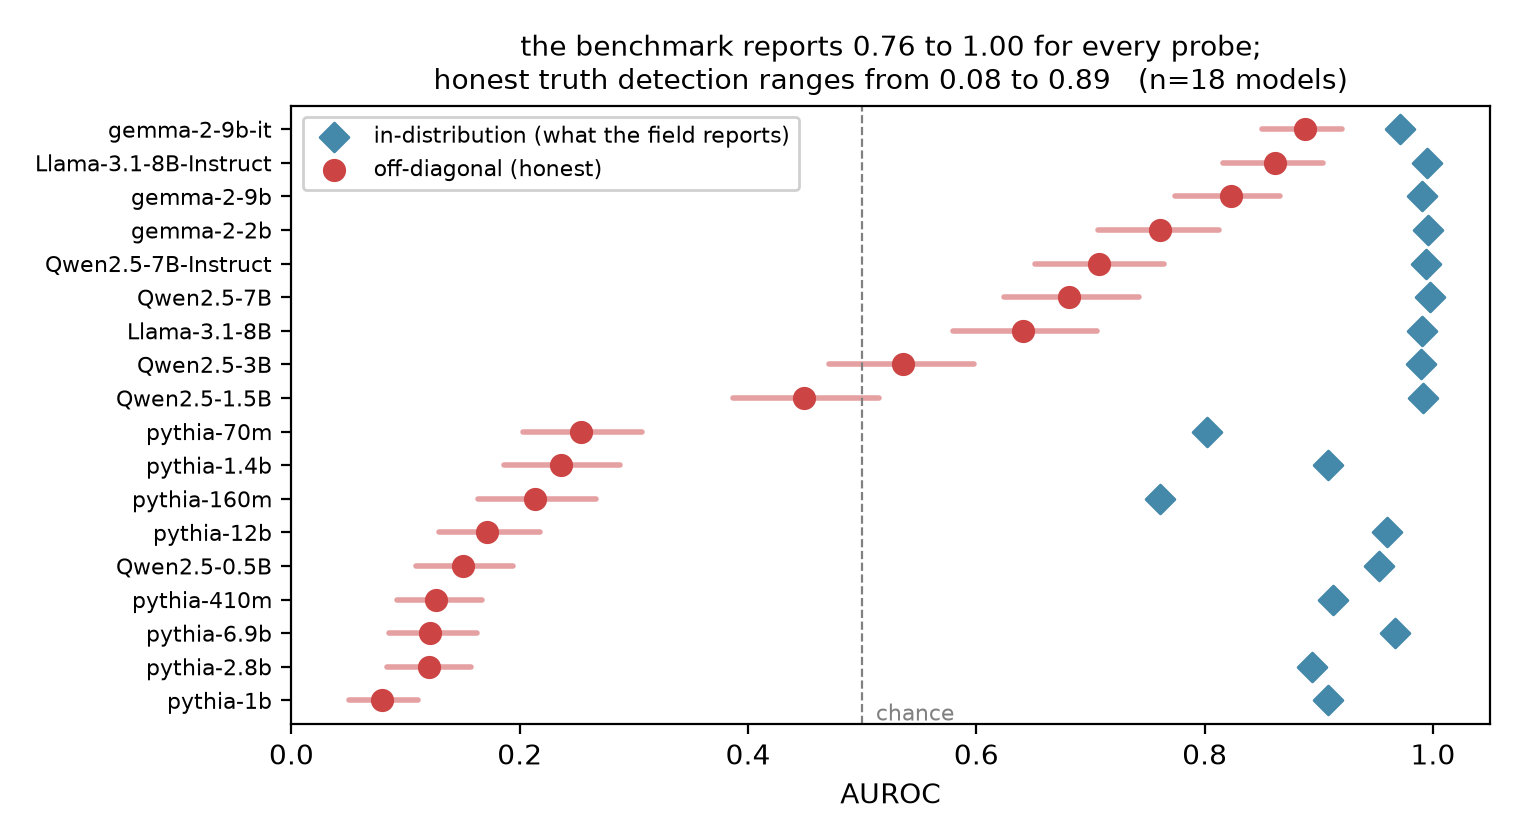
\includegraphics[width=\linewidth]{figs/fig_benchmark_blindness.png}
\caption{The benchmark reports 0.76 to 1.00 for every probe; honest truth detection ranges from 0.08 to 0.89}
\label{fig:blindness}
\end{figure}

The in-distribution column spans 0.24 of the metric. The off-diagonal column spans 0.81. Nothing measurable on the diagonal orders these probes correctly, and the two extremes, a near frequency readout and a working truth detector, are not far apart in the column the field publishes.

That is one probe family. Pooling every probe and model pair we ran, six architectures from four research groups across eighteen models, gives 98 pairs, and the question becomes whether the published number orders them at all. It does not. The in-distribution score predicts the off-diagonal AUROC at Spearman \textbf{0.198, p = 0.051, bootstrap interval [-0.005, 0.366]}, over in-distribution scores spanning 0.305 to 1.000 and off-diagonal AUROCs spanning 0.056 to 0.989. \textbf{Forty-eight of the 98 pairs fall below chance} on the off-diagonal split, the lowest being DRIFT on Qwen2.5-0.5B at 0.056. A reader choosing a detector on the reported number is choosing close to at random with respect to what it is worth off the diagonal.

Every gap is positive and every confidence interval excludes zero, including Gemma-2-9b-it at +0.083 [0.015, 0.131]. We had previously reported that model as a clean negative and we withdraw that. It was measured on a corpus where the edit shortcut alone was worth +0.075, which exceeded the effect. On the present corpus that shortcut is exactly zero and the residual is still there, so it is a real if small dependence rather than a construction artifact. What survives of the earlier claim is the ordering: the confound differs by a factor of ten between the best and worst models in this set, and at the good end it is small enough to be practically minor.

\subsection{What the failure looks like}

Mean probe score by cell, where TT and TA are true statements that should read near 1.00 and FT and FA are false ones that should read near 0.00:

\begin{table}[t]
\centering
\small
\resizebox{\linewidth}{!}{%
\begin{tabular}{lrrrrr}
\toprule
\textbf{Model} & \textbf{TT} & \textbf{TA} & \textbf{FT} & \textbf{FA} & \textbf{\emph{(mean probe score, 0-1)}} \\
\midrule
Pythia-12b & 0.934 & \textbf{0.247} & \textbf{0.711} & 0.078 &  \\
Qwen2.5-1.5B & 0.940 & 0.435 & 0.390 & 0.067 &  \\
Qwen2.5-7B & 0.959 & 0.535 & 0.218 & 0.035 &  \\
Llama-3.1-8B & 0.955 & 0.561 & 0.242 & 0.052 &  \\
Gemma-2-9b & 0.962 & 0.728 & 0.198 & 0.050 &  \\
Llama-3.1-8B-Instruct & 0.959 & 0.680 & 0.156 & 0.032 &  \\
Gemma-2-9b-it & 0.906 & 0.800 & 0.095 & 0.095 &  \\
\bottomrule
\end{tabular}}
\end{table}

Read the Pythia-12b row as one sentence: common means true, rare means false, largely regardless of the truth value. It scores 0.934 on common truths and 0.247 on rare ones, and it rates fluent falsehoods at 0.711, higher than it rates the true statements in TA. Its output is closer to entity frequency wearing a truth label than to a truth detector, and it scores 0.960 on the benchmark.

In the stronger models the rare true cell is where the damage concentrates and it is less severe, 0.535 to 0.800 rather than 0.247. Fluent falsehood is handled correctly everywhere above the small models. That asymmetry is worth stating plainly because we previously concluded the opposite: on an earlier corpus containing only strong models we reported that the fluent falsehood prediction was refuted. It is not refuted. It fails hard in exactly the models where truth is least available, and we had not tested those.

\subsection{Why it happens, and in what shape}

The last column of the results table is recoverability: how well truth can be linearly decoded from the same hidden states when the probe is trained on decorrelated data instead of the diagonal. It is a property of the representation, not of the probe.

Across the eighteen models, recoverability and off-diagonal AUROC correlate at \textbf{r = 0.821 [0.706, 0.917]}. But a correlation assumes a line and this is not one. Comparing three shapes on the same data by AIC gives linear $-$60.65, step $-$74.88, and hinge $-$90.12, so the hinge is preferred by a wide margin over both alternatives:

\begin{quote}
honest\_off = 0.164 [0.126, 0.204] + 4.81 [1.88, 7.65] × max(0, recoverability $-$ 0.765 [0.57, 0.80])
\end{quote}

\begin{figure}[t]
\centering
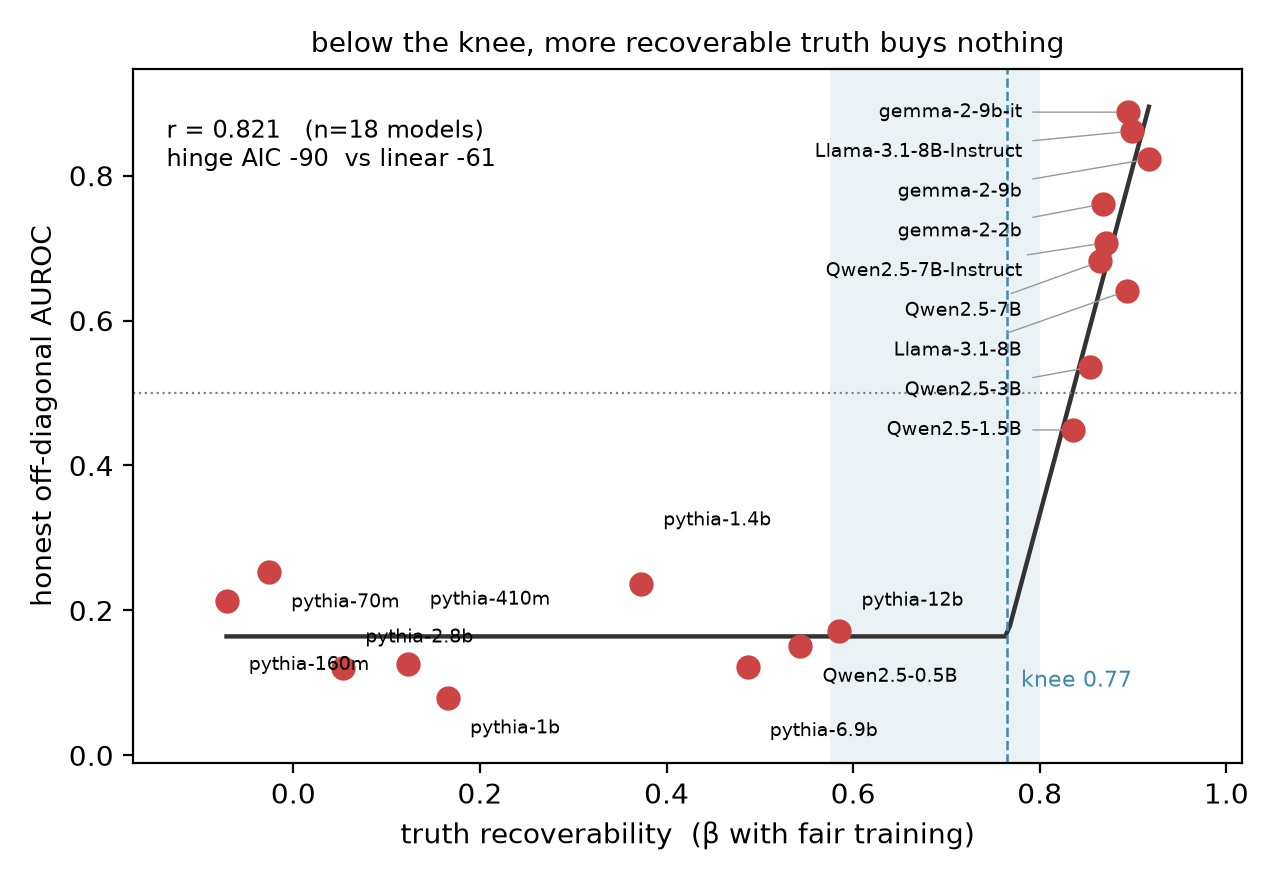
\includegraphics[width=\linewidth]{figs/fig_recoverability_mechanism.png}
\caption{Below the knee, more recoverable truth buys nothing}
\label{fig:mechanism}
\end{figure}

Below the knee, nine models spanning recoverability from $-$0.072 to 0.585 all sit between 0.079 and 0.253 honest. More recoverable truth buys them nothing whatsoever. Above the knee, off-diagonal AUROC climbs steeply. So the substitution is not proportional to how unavailable truth is, as we described it in an earlier version of this work. It is total until a threshold is crossed.

We settled the functional form with new data rather than by fit quality. At an earlier stage, with thirteen models on corpus v6206fe484650, a step function fit best and its threshold fell inside a region of recoverability where we had no models at all. Rather than adopt the better fitting shape, we ran five models chosen to land in that gap. On that corpus Qwen2.5-1.5B came back at recoverability 0.813 and honest 0.460, interpolating rather than jumping, which refuted the step. The hinge then beat both, and still does here.

The hinge shape is stable across the two most recent versions of this corpus, though its parameters are not tightly pinned: the knee moved from 0.610 to 0.765 between them and the slope interval is wide. Recoverability is also not a complete account above the knee, where Qwen2.5-3B reaches only 0.536 honest at recoverability 0.854 while Gemma-2-2b reaches 0.761 at 0.868.

It is worth saying plainly what this relation does not cover. Both of those corpora are built the same way, with falsehoods we wrote. On a corpus whose falsehoods a model produced instead, the same measurement gives a correlation of 0.490 with an interval containing zero, and the hinge is no longer preferred. That result is reported in full below. The reader should take the account in this section as describing the authored case and should not extend it to natural error.

\subsection{Scale is not the variable}

Within the Pythia family, going from 70m to 12b does not clean the probe up. Off-diagonal AUROC across that whole ladder stay between 0.079 and 0.253 while recoverability climbs from $-$0.026 to 0.585. Parameter count is not what determines whether a probe reads truth.

What moves the number is whether the model has a linearly accessible truth representation for the probe to find, which is what recoverability measures directly, and whether that representation clears the knee.

\section{What this means for practice}

A hallucination detector built this way, deployed on a model where truth is not linearly available, does not fail randomly. It fails as a function of how common the subject is. It flags true statements about less common entities and passes fluent falsehoods about famous ones, the precise inversion of what a verification tool is for, and worst on the long tail knowledge where verification matters most.

None of this is visible on the benchmark. The only way to see it is to break the correlation on purpose.

\section{The benchmark cannot select a layer either}

Every result above reads one layer per model. The literature disagrees about which layer carries truth, so we swept all of them, across eighteen models and four probe architectures, and asked what the benchmark can say about the choice.

It can say almost nothing, and the reason is saturation. Gradient trained logistic regression scores in-distribution AUROC within 0.01 of its maximum at many layers simultaneously: 37 layers on Gemma-2-9b-it, 35 on Gemma-2-9b, 29 on Llama-3.1-8B-Instruct, 22 on Qwen2.5-7B-Instruct. Across the layers it scores indistinguishably, off-diagonal AUROC ranges from 0.015 to 0.875. The benchmark returns effectively one number for layers that differ by 0.86 in what they are actually worth. Mass mean probing and TTPD mostly have a unique best layer with zero spread, because their in-distribution scores top out below 1.0 and never saturate. The benchmark loses the ability to discriminate exactly where it reports a perfect score.

Published selection rules do not rescue this. Averaged over 72 probe and model pairs, the ``earliest informative layer'' criterion, meaning the earliest layer within 95\% of the maximum in-distribution AUROC, lands on layers averaging \textbf{0.333 honest and forfeits 0.337} against the best layer available. Fixed fractional depths in the upper third of the network, as used by \citet{hussain2026parallax}, average 0.507 to 0.533. Our own mid depth choice averages 0.503, which is marginally the worst of the fixed rules, and we report that rather than presenting our layer as neutral.

\section{Five probe architectures, four research groups}

Everything above used our own SAPLMA style implementation, which leaves the obvious question: is any of this a property of our probe rather than of the corpus and the representation? We ran four published probes through the auditor, at every layer, on the same eighteen models.

\begin{table}[t]
\centering
\small
\resizebox{\linewidth}{!}{%
\begin{tabular}{lrrr}
\toprule
\textbf{Probe} & \textbf{Origin} & \textbf{Shape} & \textbf{r(our recoverability, its off-diagonal AUROC)} \\
\midrule
Logistic regression & \citet{marks2023geometry} & gradient descent, single layer & 0.859 [0.773, 0.933] \\
Mass mean & \citet{marks2023geometry} & closed form mean difference & 0.826 [0.719, 0.932] \\
TTPD & \citet{burger2024truth} & two dimensional truth subspace & 0.813 [0.672, 0.931] \\
CCS & \citet{burns2023discovering} & unsupervised, contrast consistency & 0.676 [0.515, 0.818] \\
\bottomrule
\end{tabular}}
\end{table}

\emph{Mass mean, TTPD and CCS are read at the layer the benchmark selects for each; logistic regression at our headline layer, since its in-distribution score saturates across dozens of layers and the benchmark therefore selects nothing. All four intervals exclude zero.}

TTPD matters most here. It comes from a different group, models truth as a two dimensional subspace with separate general truth and polarity directions rather than a single direction, and was designed specifically to survive negation. It tracks recoverability anyway, at 0.835 [0.727, 0.944] over the seventeen models where it has adequate signal. That is the strongest evidence we have that the relation is a property of the representation rather than of any probe family, since nothing about TTPD's construction is shared with ours.

CCS is the weakest of the four and we report it as such. It clears the 0.70 in-distribution floor on only 7 of 18 models and fails to reach it at any layer on every Pythia, so on the models where the confound is largest it cannot adjudicate at all. Restricted to the models where it is adequately powered its correlation is 0.228 [$-$0.507, 0.961], which is not distinguishable from zero at n = 7. A detector with no diagonal signal has no confound to lose, and we do not count CCS as independent confirmation.

\subsection{A multi-layer, multi-token probe is more confounded, not less}

\emph{Eight models spanning the recoverability range.}

All five probes above read a single token at a single layer, which leaves open whether the confound is a property of that shape. DRIFT (\citealp{hussain2026parallax}) is neither: it taps four upper depth layers, mean pools each over all tokens, and its features are the differences between layer pairs, so it reads how the residual stream changes with depth rather than where it sits.

It is a strong probe on our corpus, with in-distribution AUROC between 0.894 and 1.000, so its gaps are informative rather than empty. Its off-diagonal AUROC is between 0.056 and 0.523. On Gemma-2-9b-it, where the single layer probes reach 0.89 to 0.99 honest, DRIFT reaches 0.387. Recoverability predicts its off-diagonal AUROC at r = 0.477 [$-$0.098, 0.872], an interval that includes zero at eight models, so we do not claim the mechanism for DRIFT. Its own concat ablation, the same four taps without the inter layer differencing, is worse still on six of the eight. Neither variant escapes the confound, and a multi layer multi token reader is more confounded than the single layer family rather than less.

We note one plausible mechanism without testing it: mean pooling over all statement tokens gives a probe more direct access to the entity's own representation than a last token read does, which would make entity frequency easier rather than harder to pick up.

\subsection{A sampling based detector shows no frequency penalty at all}

\emph{Three instruction tuned models, 180 subjects each.}

Semantic entropy (\citealp{farquhar2024semantic}) never looks at the residual stream. It samples the model ten times, clusters the answers by bidirectional entailment with an NLI model, and measures the dispersion. On our corpus it works: it detects each model's own errors at AUROC 0.776, 0.822 and 0.758.

And restricted to statements each model got right, which is the exact contrast that exposes the probes, it separates rare true from common true at \textbf{0.514 [0.465, 0.565], 0.500 [0.440, 0.561] and 0.509 [0.474, 0.546]}. Exactly chance on all three, with every interval containing 0.5. The fielded linear probes, on the same axis, degrade from a mean score between 0.65 and 0.96 on common true statements down to between 0.14 and 0.80 on rare ones, across the eighteen models.

So the confound is a property of linear readouts of hidden states, not of the model's own uncertainty. This is the reason we scope every claim in this paper to trained probes on hidden states rather than to hallucination detection in general.

On an earlier corpus this test wobbled, with one model showing common entities carrying higher entropy than rare ones, which we attributed to shared city names returning different valid answers under sampling. That asymmetry is absent here: all three models sit within 0.015 of chance.

\section{A second corpus, with falsehoods we did not write}

Everything above rests on statements we constructed. The false ones were made by swapping an entity in a true statement, which is the standard recipe, and it is also the obvious objection: we built the thing we measured, and two of our five attempts manufactured the effect we were hunting. So we built a second corpus on a different principle and repeated the measurement.

Its false statements are mistakes a model actually made. We asked Qwen2.5-1.5B-Instruct which country each of four thousand cities is in, and kept the answers that were wrong. Nothing about those falsehoods is our choice. To decide what counts as wrong we used Wikidata rather than the knowledge base behind our other corpus, because that base lists one country per city name and is incomplete: it calls ``Barcelona is a city in Spain'' false, since its Barcelona is the Venezuelan one. Measured directly, \textbf{46\% of the errors it produced were statements that are actually true}. Wikidata gives every country hosting a city of that name, so an answer counts as an error only if it matches none of them. The result is \texttt{vd279c2cae5f4}, 140 statements, 35 per cell.

\textbf{The central finding survives, and gets stronger.} Every model still scores near the top of the benchmark, 0.875 to 1.000. On the off-diagonal test, all eighteen fall between \textbf{0.049 and 0.447}. Not one of them beats chance. Every gap is positive with an interval excluding zero, and the best performer, Gemma-2-9b, reaches 0.447 [0.31, 0.58]. On falsehoods that a model produced by itself, none of these detectors works at all, and the benchmark still reports them as near perfect.

\textbf{The mechanism does not survive.} Recoverability and off-diagonal AUROC correlate at \textbf{0.490 [$-$0.077, 0.754]}, an interval that includes zero, against 0.821 [0.706, 0.917] on the authored corpus. Model comparison no longer prefers the hinge. Gemma-2-9b-it has recoverability 0.866 here and still reaches only 0.428. So the account in the previous section describes probes reading falsehoods we wrote, and does not describe probes reading falsehoods a model wrote. We state that as a limit on the explanation rather than repairing it.

This is consistent with a smaller earlier experiment in which a probe correctly rejected our synthetic fluent lies while accepting the same model's own disowned outputs. Synthetic falsehood is detectable; natural error is not. The confound is worse in the natural case, not milder.

Three reasons to treat this corpus as provisional rather than as a second headline. Its false-and-ordinary cell is capped at 35 items, because models rarely err about famous places, and that scarcity is itself a fact about natural errors rather than a build failure. Its tokenization canary reads 0.636 [0.397, 0.866], passing only because the interval is wide at this size; country names in true statements average 8.8 characters against 7.1 in false ones, so some of the signal a probe sees here is surface form. And roughly three thousand candidate items were dropped because we could not obtain frequency counts for their entities, which is what holds the corpus at 140.

\section{The collapse is a property of the training distribution}

Every result above trains on our own diagonal, where entity frequency and truth agree because we made them agree. That is a statement about what the standard recipe does when the alignment is present. It is not a statement about the datasets the field actually uses, and the difference matters enough to test directly.

Before the result, two defects in it that we found only after first reporting it, and that a reader should weigh before reading the numbers.

The first is contamination. Our authored corpus is itself derived from files in an Azaria and Mitchell directory, so \textbf{458 of its 608 statements (75.3\%) appear verbatim in them}, labels included. A first version of this experiment trained on all 16,329 rows and reported near-perfect transfer, which was memorization of the evaluation set. We now exclude every training row whose subject entity appears anywhere in either corpus, which drops 6,882 rows, and 177 exact duplicates, leaving \textbf{9,270 statements, 49.3\% true}. All numbers below are from the decontaminated fit.

The second is provenance, and it is not fully repaired. We fetched the published artifact (\texttt{true-false-dataset.zip}, sha256 \texttt{f21fa017...}) and compared it against the directory we had trained on. Three files are byte-identical, and the official \texttt{cities\_true\_false.csv} is byte-identical to a file we held under the name \texttt{capitals\_true\_false.csv}. But the \texttt{cities\_true\_false.csv} in our directory holds \textbf{10,000 rows and does not appear in the published artifact at all}, overlapping the official cities file by 397 rows; \texttt{companies} differs in 398 of 1,200 parsed rows, \texttt{elements} in 2 of 930, and \texttt{facts} is a different version. So the directory is a modified derivative of that release, assembled before this work began, and its largest file is of unidentified origin. Our corpus generator reads that file for its cities domain, which is 304 of our 608 authored items.

Two consequences, stated rather than resolved. The numbers in this section describe a derivative and \textbf{we do not attribute them to Azaria and Mitchell}; the rerun on the published artifact is the obvious next experiment and is not in this paper. And the left-hand anchor of the alignment spectrum, the claim that a published dataset carries the confound only partially, rests on that same derivative and should be read as provisional.

Trained this way, at each model's mid-depth layer, and applied unchanged to our corpora, the probe does not collapse on our authored off-diagonal.

\begin{table}[t]
\centering
\small
\resizebox{\linewidth}{!}{%
\begin{tabular}{lrrr}
\toprule
\textbf{model} & \textbf{A\&M held-out (AUROC)} & \textbf{our off-diagonal (AUROC)} & \textbf{frequency read among true items only (AUROC)} \\
\midrule
pythia-6.9b & 0.880 & 0.882 & 0.639 [0.576, 0.701] \\
Qwen2.5-7B-Instruct & 0.957 & 0.993 & 0.585 [0.524, 0.645] \\
Llama-3.1-8B-Instruct & 0.971 & 0.997 & 0.620 [0.555, 0.683] \\
gemma-2-9b-it & 0.978 & 0.997 & 0.588 [0.526, 0.651] \\
\bottomrule
\end{tabular}}
\end{table}

So the 0.08 floor reported earlier is caused by the training composition we impose, not by the method. Frequency reading is much reduced relative to our diagonal-trained probes, which reach 0.766 to 0.961 on the same contrast, but it is not removed: every interval here excludes 0.5.

The second half of the experiment is less comfortable for the method. Holding the probe weights fixed and changing only which corpus supplies the false-common cell. These are mean probe scores on a zero-to-one scale, not AUROC.

\begin{table}[t]
\centering
\small
\resizebox{\linewidth}{!}{%
\begin{tabular}{lrrrr}
\toprule
\textbf{model} & \textbf{authored false-common (mean score)} & \textbf{harvested false-common (mean score)} & \textbf{harvested off-diagonal (AUROC)} & \textbf{harvested frequency read (AUROC)} \\
\midrule
pythia-6.9b & 0.126 & 0.487 & 0.606 & 0.891 [0.806, 0.961] \\
Qwen2.5-7B-Instruct & 0.014 & 0.491 & 0.858 & 0.667 [0.519, 0.796] \\
Llama-3.1-8B-Instruct & 0.022 & 0.287 & 0.908 & 0.581 [0.424, 0.732] \\
gemma-2-9b-it & 0.034 & 0.556 & 0.899 & 0.642 [0.502, 0.773] \\
\bottomrule
\end{tabular}}
\end{table}

Our authored false-common items are made by swapping a country, which is how Azaria and Mitchell's false statements are made too. The probe rejects them at 0.014 to 0.126. The harvested items are wrong answers a model produced, and the same weights place them at 0.287 to 0.556, which is indifference rather than rejection. The probe is confident about falsehoods built the way its training falsehoods were built and has close to no opinion about falsehoods it has not seen constructed. That gap is present in all four models and is the finding here with a deployment consequence.

Frequency reading is reduced by training on their data but not removed, and on pythia-6.9b it is not reduced at all: 0.891 [0.806, 0.961] among true-only harvested items, with the lowest off-diagonal score of the four at 0.606. A quarter of this sample therefore reads frequency about as hard after training on their data as our own probes do after training on ours, so ``training on their data does not teach the shortcut'' holds for three of four models and not as a general claim. Four models cannot settle it either way; extraction over the training set costs roughly fifteen times a corpus pass, which is why this is four and not eighteen.

Two further limits. Their released files contain cities, companies and inventions statements close to our sentence pattern, so this is transfer between neighbours and not a test of distant generalization, which makes the off-diagonal column a weak upper bound rather than evidence of a general capability. And the two runs give pythia-6.9b a held-out score of 0.880 and 0.881, and Llama-3.1-8B-Instruct 0.971 and 0.972, from identical data and seed. That is the size of the half-precision extraction noise, so differences below about 0.003 anywhere in this paper are ties and no claim here rests on one.

\section{The tool}

We release what we used to check ourselves, because four of our own corpora failed and the checks that caught them are cheap.

The corpus auditor takes any candidate decorrelation corpus and runs seven checks: crossing, FT yield, composition, duplicates, domain share, edit balance, and given a GPU the two hidden state canaries. Run against our own history it flags the first corpus on composition, duplicates and domain share, flags the third on duplicates, flags the fourth on edit balance, and clears the fifth. A tool that cannot catch its author's mistakes will not catch anyone else's.

The probe auditor takes any detector with \texttt{fit} and \texttt{score} and returns the triple this paper argues every such paper should publish: headline, controlled, and the gap with a bootstrap interval, plus the per cell breakdown. It is symmetric by construction and tested to be: the suite builds one confounded probe and one honest probe and requires the tool to flag the first and clear the second.

We also suggest reporting a second interval that this literature does not. The usual bootstrap resamples the evaluation set with the fitted probe held fixed, so it cannot see instability in the fit itself. Refitting on repeated 90\% subsamples shows that this matters for some architectures and not others: gradient trained logistic regression gives refit ranges that closely match its evaluation intervals, while mass mean probing on Pythia-1.4b moves across [+0.045, +0.586] where its reported interval is [+0.373, +0.593].

\subsection{Gates for experiments, not just for corpora}

The corpus gates above were built because four corpora failed. Every experiment in this paper then ran outside any equivalent check, and one of them failed the same way.

The transfer experiment in the previous section was first run without excluding our evaluation items from its training set. It reported near-perfect transfer, and that number was memorization: three quarters of the evaluation corpus sat in the training data because both derive from the same files. It was written into a draft of this paper as a headline correction before anyone noticed. What caught it was not a check and not a rerun. It was a reader noticing that a row count, 16,329, did not match the count in the paper the data was attributed to.

We record this because the moral is the paper's own thesis applied to us. We were auditing shortcut contamination, and shipped a contaminated experiment, in the section about contamination, caught by manual reading rather than by any gate. Reading does not scale and does not run twice. So the released tooling carries two registers rather than one:

\begin{itemize}
\item \textbf{Corpus gates}, the five described above, which run inside \texttt{finalize()} and refuse to write a corpus that fails.
\item \textbf{Experiment gates}, which are new: entity-level exclusion between any training set and any evaluation set, and a provenance manifest recording source URL, retrieval date, sha256 and expected row count for every file under \texttt{data/}. A manifest makes a 10,000-row file in a slot that should hold 1,458 impossible to not notice, which is the specific failure that cost us this experiment.
\end{itemize}

\section{Compute}

Everything reported here runs on a single GPU per job. The target in our own project directive is one A10G or L4 class card, on the argument that rigour rather than scale is the constraint in this kind of audit, and nothing in the paper needed more: the largest model is 9B in bfloat16, roughly 18GB of weights, which fits in 24GB with headroom for batched activation extraction. Part of the work was run on H100 purely for speed, and the final layer sweep was run on A10G after a workspace lost H100 entitlement, with no change to any result.

\begin{table}[t]
\centering
\small
\resizebox{\linewidth}{!}{%
\begin{tabular}{lr}
\toprule
\textbf{Quantity} & \textbf{Value} \\
\midrule
Distinct models & 18, from 70M to 12B parameters, four families \\
Committed GPU run artifacts & 150 \\
Stage 3 runs (the main sweep) & 49 \\
All layer, all probe sweeps & 46 \\
Corpus builds reaching the gates & 5 \\
Corpus versions released & 5, of which 4 withdrawn \\
GPU classes used & H100 and A10G, one card per job \\
\bottomrule
\end{tabular}}
\end{table}

The single most expensive operation is hidden state extraction, which is why activations are cached per model and corpus and reused across the per layer analyses. A full eighteen model Stage 3 sweep on one corpus completes in well under an hour of wall clock when jobs run concurrently, since each job handles one model.

\textbf{We cannot give an exact GPU hour or dollar total, and we would rather say so than estimate one.} No runtime was recorded in the artifacts until the final stage of this work, and the project moved through five separate cloud workspaces as prepaid credits were exhausted, three of which are no longer accessible, so the billing history is not recoverable. This is a reporting failure on our part rather than a small omission: a compute budget is exactly the kind of number a reader should be able to check, and ours is not checkable for the historical runs. Every run from the final stage onward records its wall clock seconds and GPU class into its artifact, so this is measurable going forward. We note the cost of the retractions specifically: four of the five corpora were rebuilt after a defect was found, and each rebuild invalidated every downstream result on that corpus, so a substantial fraction of the total compute bought results that are not in this paper.

\section{Where it is thin}

Three domains, English, one template family per domain, and all of them subject object factual statements. Whether this holds for multi clause claims, reasoning chains, or open generation is untested.

n = 608 is small, and smaller than our previous corpus at 720. It shrank because balancing edit provenance inside every cell costs items, and we would rather report 608 statements with no exploitable construction shortcut than 720 with one worth 0.075.

\textbf{The main corpus is built by one pipeline}, with falsehoods authored by entity swap, typicality from a single frequency source, and gates of our own design. Breadth alone would not fix that: more domains through the same generator multiplies the same construction choices. We therefore built the second corpus described above, whose falsehoods come from a model's own errors and whose labels come from an external gazetteer. The central claim replicates there and in fact strengthens, which is the outcome that matters most; the explanatory account does not replicate, which we report rather than resolve.

That second corpus is small (n = 140) and provisional for the reasons given in its section, so it should be read as a first independent check rather than a settled replication. A larger version, and a corpus taken from another group entirely, would both strengthen the case further. Given that two of our five corpora manufactured the very effect we were hunting, corpus provenance remains the limitation a reader should weigh most heavily.

\textbf{Half the authored corpus rests on a file we cannot name.} The cities domain, 304 of 608 items, is generated from the 10,000-row file described above, which is not part of the published artifact it was filed under. We verified its labels against Wikidata rather than trusting them: of 255 checkable city items, 12 disagree, and inspection attributes ten to gaps in the gazetteer (Altay, Sale, Braila, Mbabane, Praia, Mbandaka are all real cities whose country Wikidata did not return under the queried name).

The remaining two disagreements are the direction that matters and reveal a design flaw rather than a data error. \emph{Santiago is a city in Mexico} and \emph{Geneva is a city in United States} are both labelled false in our false-common cell, and both are probably true. The mechanism is systematic: that cell is built by swapping a country into a \textbf{common} city name, and common city names are exactly the ones with namesakes worldwide, so the swap can land on a truth. The risk concentrates by construction in the one cell the paper's argument depends on. Wikidata's coverage is incomplete, so 2 of 255 is a floor rather than an estimate. The fix is a build gate rejecting any swapped pair that a multi-valued gazetteer attests, it is not in the released gates yet, and until it is the false-common cell should be read as containing an unknown but small number of true statements. This works against the effect we report rather than for it: true statements sitting in the false cell make a truth-reading probe look worse, not better.

\textbf{The transfer experiment is four models on a derivative.} It is the evidence for the paper's scope claim, that the collapse depends on training composition, and it is the thinnest result here: four models rather than eighteen, mid-depth rather than each model's headline layer, and on the unverified directory rather than the published dataset. Its own frequency-reading column disagrees across those four, with pythia-6.9b at 0.891 against 0.581 to 0.667 for the rest, so the sample cannot settle the general claim in either direction.

Recoverability is measured as a linear readout, the same shape as most of the probes. That it also predicts DRIFT, which is neither single layer nor single token, rules out the narrow version of that circularity, but not every version.

TTPD is our reimplementation from the published equations rather than the authors' code, which we could not retrieve, and is validated on synthetic activations where both directions are known by construction. Its provenance is weaker than the other adapters, which are vendored unmodified.

Our EigenScore variant reads truth too poorly on this corpus to adjudicate anything, and we report it as inconclusive rather than as a negative result.

\section{Related work}

That internal state probes read something other than truth has been observed before. \citet{levinstein2023still} show they fail on negation and generalise poorly. \citet{farquhar2023challenges} show unsupervised probes latch onto salient non knowledge features. \citet{cheang2026really} give a mechanistic account on which probes track parametric knowledge recall. \citet{seo2026quantifying} decompose benchmark performance by question side information and find heavy shortcut exploitation.

\citet{hussain2026parallax} are closest in spirit and complementary in substance. They show that four of six popular hallucination benchmarks embed the reference answer in the prompt, so a text similarity baseline with no access to model internals reaches 0.98 AUROC on HaluEval. Their artifact is lexical and lives in existing corpora; ours is distributional and required building a corpus to expose. Both point at the same conclusion from different directions, that reported progress in this area is substantially benchmark construction. We adopt their layer taps and their DRIFT probe here, and note that they find SAPLMA the strongest artifact free method among prior published work, which is consistent with our finding that these probes are good precisely when the representation supports them.

We differ from all of these in what we measure. Those results establish that a confound exists. We quantify how much of a reported number it accounts for, on a corpus verified to decorrelate the axis and gated against five construction failures we committed ourselves, and we show that the reported number carries little information about the answer: 0.76 to 1.00 in-distribution across probes whose off-diagonal range is 0.08 to 0.89. The hinge relation, the identification of frequency as the substituted feature, the layer selection result, and the released gates are, as far as we can find, new.

\section{Conclusion}

A probe reading hidden states can score 0.76 to 1.00 on the evaluation this field publishes while ranging from 0.08 to 0.89 at the task it claims to perform, and across 98 probe-model pairs the first number predicts the second at Spearman 0.198 with an interval containing zero. That is the result. It does not say the probes are broken, because some of them work: Gemma-2-9b-it reaches 0.888 honest. It says the published number does not tell you which.

What the probe substitutes when truth is not linearly available is entity frequency, and we can measure that directly by deleting every false statement and asking the probe to sort common from rare, where it scores 0.766 to 0.961 with truth held constant. The substitution is not gradual. Below a threshold in how recoverable truth is from the representation, additional recoverability buys nothing at all, and that account holds for falsehoods we wrote and fails for falsehoods a model produced.

The alignment between truth and familiarity is a spectrum rather than a property some datasets have and others lack, and the protocol reports the same high number across all of it. That is why we think the contribution has to be a gate rather than a finding. Four of our five corpora manufactured some version of the effect we were hunting, and one of our experiments trained on its own evaluation set and was caught by a reader noticing a row count. Neither was caught by being careful. Both would have been caught by a check that runs every time.
\bibliography{references}
\bibliographystyle{tmlr}

\end{document}
